\documentclass[final,times,twocolumn,5p]{ResumenEjecutivo}
\usepackage[fixlanguage]{babelbib}
\usepackage{ResumenEjecutivo}
\usepackage[none]{hyphenat}
\usepackage{amsmath}
\usepackage{algorithm}
\usepackage{algorithmic}
\usepackage{booktabs}
\usepackage{array}
\usepackage{listings}
\usepackage{xcolor}

% Configuración de lstlisting para C++
\lstset{
    language=C++,
    basicstyle=\footnotesize\ttfamily, % Tamaño de fuente pequeño y estilo monoespaciado
    columns=fullflexible, % Ajuste automático del ancho de columna
    %frame=single, % Borde alrededor del código
    breaklines=true, % Divide líneas largas automáticamente
    postbreak=\mbox{\textcolor{red}{$\hookrightarrow$}\space}, % Indicador de línea continua
    xleftmargin=1em, % Margen izquierdo para separar del texto
    backgroundcolor=\color{lightgray!20}, % Fondo suave para distinguir el código
    tabsize=4, % Tamaño de tabulación
    keywordstyle=\color{blue}, % Color para palabras clave
    commentstyle=\color{green!60!black}, % Color para comentarios
    stringstyle=\color{orange} % Color para cadenas
}
\lstdefinelanguage{Arduino}{
  language=C++,
  morekeywords={pinMode, digitalWrite, digitalRead, analogRead, analogWrite, delay, millis, loop, setup},
  sensitive=true,
  morecomment=[l]{//},
  morecomment=[s]{/*}{*/},
  morestring=[b]",
}

\lstset{
  language=Arduino,
  basicstyle=\ttfamily\small,
  keywordstyle=\color{blue},
  commentstyle=\color{gray},
  stringstyle=\color{orange},
  numbers=left,
  numberstyle=\tiny\color{gray},
  stepnumber=1,
  numbersep=5pt,
  backgroundcolor=\color{white},
  showspaces=false,
  showstringspaces=false,
  showtabs=false,
  frame=single,
  breaklines=true,
  breakatwhitespace=true,
  tabsize=2,
  captionpos=b
}


% Configuración de lstlisting para ASM
\lstdefinelanguage{Assembler}{
    alsoletter={.}, % Para reconocer etiquetas y directivas
    morekeywords={mov, add, sub, mul, div, jmp, call, ret, push, pop, cmp, je, jne, jg, jl, jge, jle, and, or, xor, not, shl, shr},
    keywordstyle=\color{purple}\bfseries,
    morecomment=[l]{;}, % Comentarios en ASM comienzan con ;
    commentstyle=\color{green!60!black},
    morestring=[b]", % Cadenas de texto entre comillas
}

\lstset{
    language=Assembler,
    basicstyle=\footnotesize\ttfamily,
    columns=fullflexible,
    breaklines=true,
    postbreak=\mbox{\textcolor{red}{$\hookrightarrow$}\space},
    xleftmargin=1em,
    backgroundcolor=\color{lightgray!20},
    numbers=left,
    numberstyle=\tiny\color{gray},
    stepnumber=1,
    tabsize=4
}

\begin{document}
\begin{frontmatter}

%----Digite el título del TFG------%
\titulo{Control de un Robot Balancín (Péndulo Invertido) Mediante Retroalimentación de Estados}

%-- Autores y direcciones --%
\author[dir1]{Lucas Pin\fnref{nota1}}
\author[dir1]{Matteo Martinez \fnref{nota2}}
\author[dir1]{Franco de Vargas\fnref{nota3}}
\address[dir1]{Estudiante de Ingeniería Mecatrónica, Facultad de Ingeniería, Universidad Nacional de Asunción, CITEC-Luque, Paraguay}

\author[dir2]{Dr. Ing. Leonardo Comparatore\fnref{nota2}}
\author[dir2]{MSc. Ing. Christian Medina\fnref{nota2}}
\author[dir2]{MSc. Ing. Paola Maidana\fnref{nota2}}

\address[dir2]{Orientador, Facultad de Ingeniería, Universidad Nacional de Asunción, CITEC-Luque, Paraguay}


%---- Palabras claves-------%
\begin{palabrasclave} 
\sep Control Optimo
\sep LQR
\sep Servo Sistema
\sep Pendulo Invertido
%% Plabras claves en el formato: palabra \sep otrapalabra
\end{palabrasclave}


\begin{resumen}
Se desarrolla el modelado y control de un robot balancín, considerado como un péndulo invertido sobre ruedas. Se parte de la obtención del modelo dinámico mediante la formulación de Lagrange, representando el sistema como cuerpos rígidos acoplados. Luego, se diseña un controlador óptimo LQR basado en realimentación de estados, con el objetivo de estabilizar la posición vertical del sistema. Finalmente, se valida el desempeño del controlador en simulación, demostrando su efectividad ante distintas condiciones iniciales.
\end{resumen}
\end{frontmatter}
\pagestyle{fancy}

\section{Introducción}
``¡Contempla, caminante del filo, la danza de un cuerpo erguido contra la tiranía de la gravedad!''.\\

El control de sistemas inestables ha sido un tema central en la teoría de control moderno, destacando el péndulo invertido como uno de los problemas más representativos por su naturaleza altamente no lineal y su inestabilidad inherente. En este contexto, el robot balancín, también conocido como self-balancing robot, ofrece una excelente plataforma para estudiar técnicas de control avanzadas aplicadas a un sistema real.

El objetivo principal de este trabajo es diseñar e implementar un controlador que permita mantener el equilibrio de un robot de dos ruedas con estructura vertical, utilizando retroalimentación de estados. Para ello, se parte de un modelado físico detallado de la planta, representando las distintas masas y componentes mecánicos como cuerpos rígidos acoplados. A partir de este modelo, se derivan las ecuaciones dinámicas mediante el método de Lagrange-Euler, identificando las principales variables de estado que influyen en el comportamiento del sistema.

Una vez modelado el sistema, se procede al diseño de un controlador óptimo mediante la técnica LQR (Linear Quadratic Regulator), que busca minimizar una función de costo cuadrática asociada al desempeño del sistema. 

La implementación física se realizó sobre plataforma Arduino, incorporando sensores como giroscopio, acelerómetro y tacómetros para estimar las variables de estado. El control se aplicó con un driver L298N usando señal PWM. 

Finalmente, se validan los resultados obtenidos tanto en simulaciones como en la implementación física del prototipo, evaluando la efectividad del control ante distintas condiciones de operación.

\section{Descripción de la Planta y Modelado Matemático}
\subsection{Descripción de la Planta} 
El fenómeno físico del robot balancín se aproxima como un modelo de cuerpos rígidos acoplados, el cual consisten en dos cilindros huecos que pueden girar completamente sobre su eje (representando las ruedas), y tres prismas de masa $m_1$, $m_2$ y $m_3$ (figura 1), donde la distancia perpendicular fija desde el centro de masa de estos prismas respecto al eje donde giran las ruedas (siendo este la referencia $y=0$) esta dado por $h_1$, $h_2$ y $h_3$, como se observa en la figura 2.
\begin{figure}[H]
    \centering
    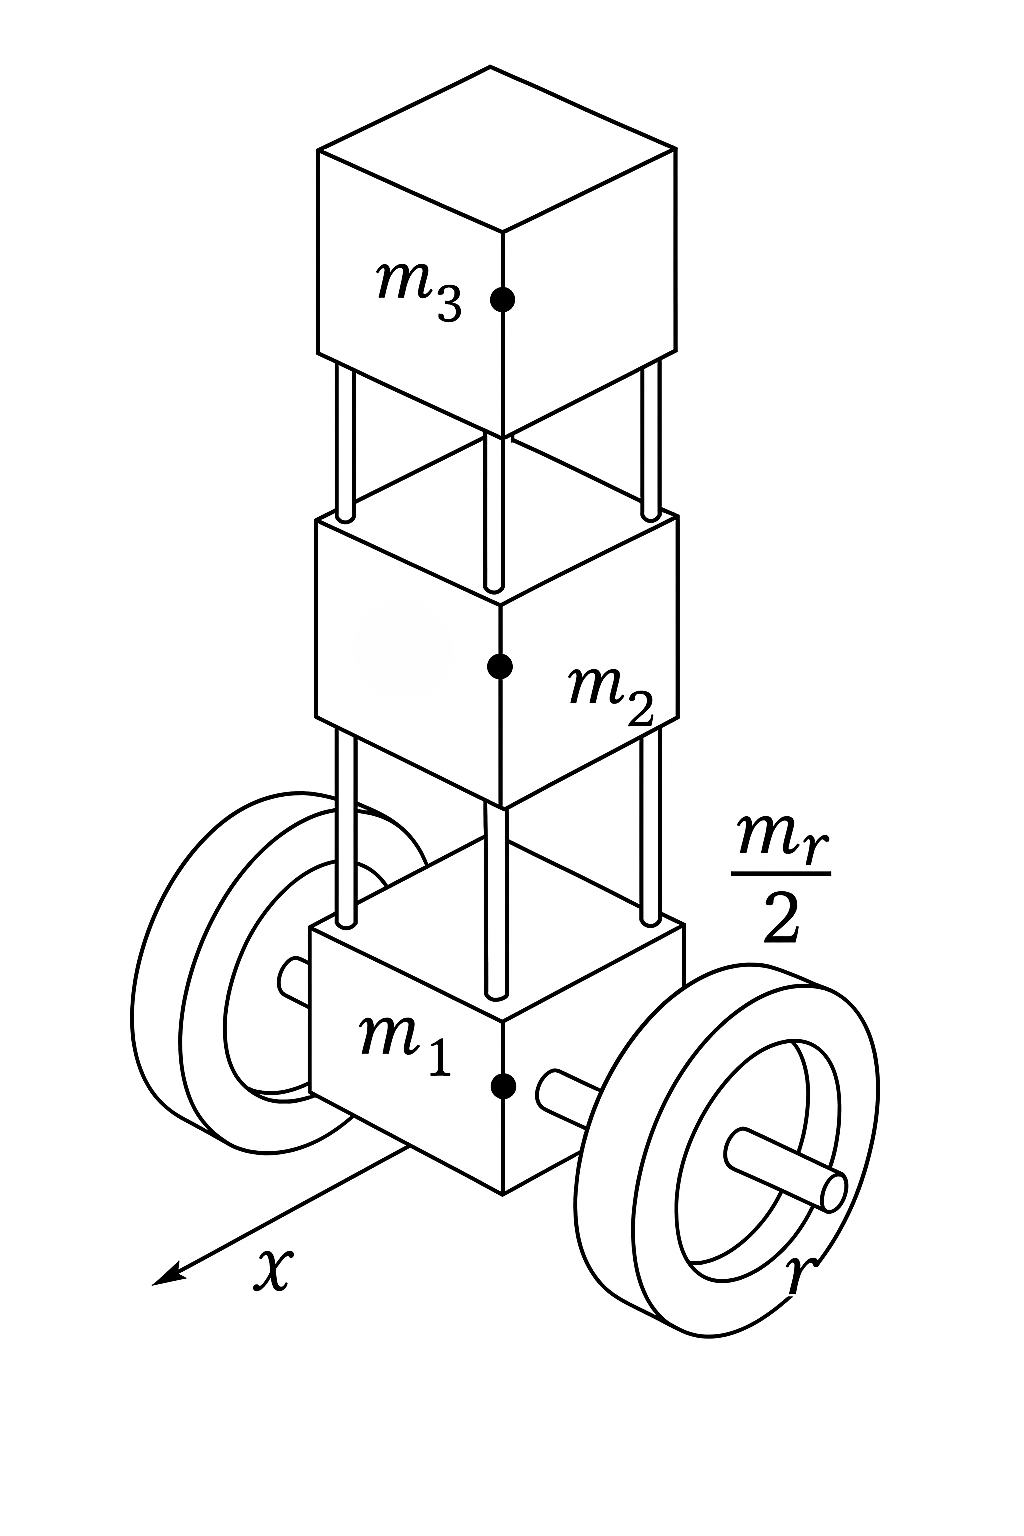
\includegraphics[width=0.5\linewidth]{imagenes/Paco_2.png}
    \caption{Esquema Tridimensional de la Planta.}
    \label{fig:enter-label}
\end{figure}
Las consideraciones tomadas para obtener sus ecuaciones dinámicas son: 
\begin{itemize}
    \item Los cilindros ruedan sin deslizar y ademas ambos tienen el mismo desplazamiento lineal en todo momento.
    \item El eje de los cilindros y los primas están acoplados rígidamente entre si.
    \item La distribución de masas esta simétricamente distribuido tal que el centro de masas de los cilindros queda en un plano normal al eje de las ruedas que pasa por el punto medio del mismo.
\end{itemize}

Estas suposiciones permiten limitar la dinámica del fenómeno a un movimiento bidimensional.

\subsection{Modelado Matemático por las ecuaciones de Lagrange-Euler}

Para obtener las ecuaciones de su dinámica de movimiento se empleo la formulación de Langrange-Euler. Las coordenadas generalizadas para este enfoque fueron tomadas como $q_1=x$ y $q_2=\theta$, donde $x$ es la distancia horizontal de del centro del eje de  las ruedas y $\theta$ es el angulo del péndulo medido desde la vertical, como se observa en la figura 2.\\
\begin{figure}[H]
    \centering
    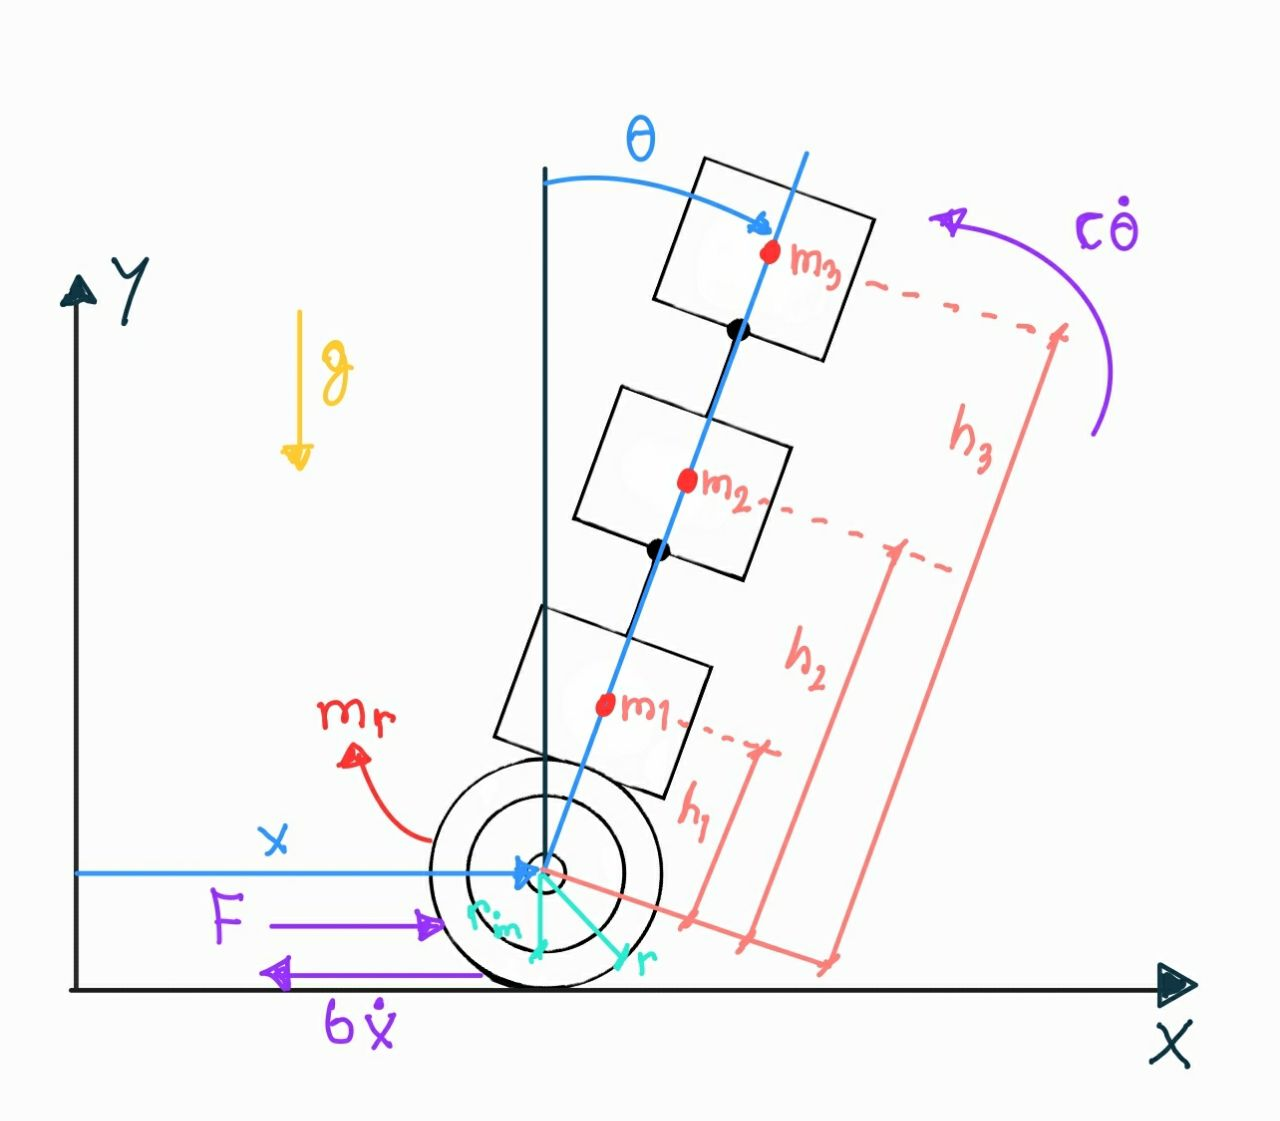
\includegraphics[width=1\linewidth]{imagenes/Modelo_2D.jpg}
    \caption{Esquema Simplificado en el Plano.}
    \label{fig:enter-label}
\end{figure}
\textit{Obtención de la Expresión de la Energía Cinética:}\\

$\Rightarrow$ Energía Cinética de las ruedas (ruedas en rotación sin deslizamiento):\\
\vspace{-0.6cm}
\begin{itemize}
    \item Masa de Cada Rueda: $m_r/2$.
    \vspace{-0.2cm}
    \item Energía transaccional: $\frac{1}{2}(m_r/2) \dot{x}^2$.
    \vspace{-0.2cm}
    \item Energía rotacional (eje propio): $\frac{1}{2}I_r (\dot{x}/r)^2$, con $I_r=\frac{1}{2}(m_r/2)(r+r_{int})^2$.
\end{itemize}
Entonces la energía cinética de las ruedas está dada por
\[
T_{ruedas} = \displaystyle 2\left[\frac{1}{2}\cdot\frac{m_r}{2}\dot{x}^2+\frac{1}{2}\cdot\frac{1}{2}\cdot\frac{m_r}{2}r^2\cdot\left(\frac{\dot{x}}{r}\right)^2\right]=\frac{3}{4}m_r\dot{x}^2
\]

$\Rightarrow$ Energía de la estructura de prismas (plataformas)\\
Para cada prisma (plataforma) $i\in \{1,2,3\}:$\\
\vspace{-0.6cm}
\begin{itemize}
    \item  Masa: $m_i$.
    \vspace{-0.2cm}
    \item Distancia del CM al centro del eje de las ruedas: $h_i$.
    \vspace{-0.2cm}
    \item Posición del CM: $x_i=x+h_isen(\theta)$, $y_i=h_icos(\theta)$.
    \vspace{-0.2cm}
    \item Velocidad total del CM:
    \[
    v_i = \displaystyle\left(\frac{dx_i}{dt}\right)^2+\left(\frac{dy_i}{dt}\right)^2= \left(\dot{x}+h_icos(\theta)\dot{\theta}\right)^2+\left(-h_isen(\theta)\dot{\theta}\right)^2
\]
\end{itemize}
Desarrollando la expresión: 
\[
v_i = \displaystyle\dot{x}^2+2h_i\dot{x}\dot{\theta}cos(\theta)+h_i^2\dot{\theta}^2
\]
Entonces, energía cinética total de los prismas es:
\[
T_{prismas} = \displaystyle\sum^3_{i=1}\frac{1}{2}m_iv_i^2
\]
\[
T_{prismas} = \displaystyle\frac{1}{2}\left(\dot{x}^2\sum^3_{i=1}m_i+2\dot{x}\dot{\theta}cos(\theta)\sum^3_{i=1}m_ih_i+\dot{\theta}^2\sum^3_{i=1}m_ih_i^2\right)
\]

Donde: \\
\vspace{-0.6cm}
\begin{itemize}
    \item $m_T=\sum m_i$.
    \vspace{-0.2cm}
    \item $M_h=\sum m_ih_i$.
    \vspace{-0.2cm}
    \item $I_h=\sum m_ih_i^2$.
\end{itemize}

$\Rightarrow$ Energía Cinética Total del Sistema:\\
\[
T = T_{ruedas}+T_{prismas}
\]
\[
T = \displaystyle\frac{1}{2}\left(m_T+\frac{3}{2}m_r\right)\dot{x}^2+M_h\dot{x}\dot{\theta}cos(\theta)+\frac{1}{2}I_h\dot{\theta}^2
\]

\textit{Obtención de la Expresión de la Energía Potencial:}\\

Para el sistema considerado, la energía potencial estada solo por la energía potencial gravitacional de las masas, esto es:
\[
V = \displaystyle\sum^3_{i=1}m_ih_ig\cdot cos(\theta)=C_1cos(\theta)
\]

Donde $g$ es la aceleración debido a la gravedad y $C_1=\sum m_ih_ig$.\\

\textit{Obtención del Lagrangiano:}\\

El Lagrangiano esta dado por:
\[
\mathcal{L} = T - V
\]
Entonces:
\[
\mathcal{L} =  \displaystyle\frac{1}{2}M\dot{x}^2+M_h\dot{x}\dot{\theta}cos(\theta)+\frac{1}{2}I_h\dot{\theta}^2-C_1cos(\theta)
\]

Donde $M=\left(m_T+\frac{3}{2}m_r\right)$\\

\textit{Ecuaciones de Lagrange-Euler:}\\

$\Rightarrow$ Para $q_1=x$
\[
\displaystyle\frac{d}{dt}\left(\frac{\partial\mathcal{L}}{\partial\dot{x}}\right)-\frac{\partial\mathcal{L}}{\partial x} =  -b\dot{x}+F
\]
Donde $b$ es fricción lineal y $F$ la fuerza neta aplicada en $x$.\\

$\Rightarrow$ Para $q_2=\theta$
\[
\displaystyle\frac{d}{dt}\left(\frac{\partial\mathcal{L}}{\partial\dot{\theta}}\right)-\frac{\partial\mathcal{L}}{\partial\theta} =  -c\dot{\theta}
\]
Donde $c$ es la fricción angular.\\

\textit{Ecuaciones de Movimiento del Sistema:}
\[
\fbox{
  $\begin{aligned}
  (1) \quad M\ddot{x} + M_hcos(\theta)\ddot{\theta}&= F-b\dot{x}+M_hsin(\theta)\dot{\theta}^2 \\
  (2) \quad I_h\ddot{\theta} +M_hcos(\theta)\ddot{x}&= C_1sen(\theta)-c\dot{\theta}
  \end{aligned}$
}
\]

\textit{Linealización del Sistema:}\\

Para poder llevar la expresión de la planta al espacio de estados, se requiere de una linealización previa. Considerando la linealización al redero del punto de equilibrio $\theta=0$, se tiene:
\vspace{-0.6cm}
\begin{itemize}
    \item $cos(\theta)\approx1$.
    \vspace{-0.2cm}
    \item $sen(\theta)\approx\theta$.
    \vspace{-0.2cm}
    \item $\dot{\theta}^2\approx0$.
\end{itemize}

Entonces, el sistema linealizado queda como:
\[
\fbox{
  $\begin{aligned}
  (1') \quad M\ddot{x} + M_h\ddot{\theta}&= F-b\dot{x}\\
  (2') \quad I_h\ddot{\theta} +M_h\ddot{x}&= C_1\theta-c\dot{\theta}
  \end{aligned}$
}
\]

Tomando los estados como:
\[
X=
\begin{bmatrix}
x_1&x_2&x_3&x_4 
\end{bmatrix}^T
=\begin{bmatrix}
x&\dot{x}&\theta&\dot{\theta} 
\end{bmatrix}^T
\]

Es necesario conseguir las variables $\ddot{x}$ y $\ddot{\theta}$ de $(1')$ y $(2')$ en función de las variables de estados $x_1,\;x_2,\;x_3$ y $x_4$. Esto es posible resolviendo la ecuacion matrical dada por:
\[
\begin{bmatrix}
M & M_h \\
M_h & I_h \\
\end{bmatrix}\\
\begin{bmatrix}
\ddot{x}\\
\ddot{\theta} \\
\end{bmatrix} =
\begin{bmatrix}
F-c\dot{x}\\
C_1\theta-c\dot{\theta} \\
\end{bmatrix}
\]

Dando como resultado: 
\[
  \begin{aligned}
  \ddot{x}&=\displaystyle-\frac{I_hb}{\Delta}\dot{x}+\frac{M_hC_1}{\Delta}\theta-\frac{M_hc}{\Delta}\dot{\theta}+\frac{I_h}{\Delta}u\\
  \ddot{\theta}&= \displaystyle\frac{M_hb}{\Delta}\dot{x}+\frac{MC_1}{\Delta}\theta-\frac{Mc}{\Delta}\dot{\theta}-\frac{M_h}{\Delta}u\\
  \end{aligned}
\]
Donde:
\begin{itemize}
    \item $\Delta=MI_h-M_h^2$ y $F=u$ el esfuerzo de control.\\
\end{itemize}

\textit{Forma en el Espacio de Estados:}\\
\[
X=A\dot{X}+Bu
\]

Donde las matrices $A$ y $B$ están dadas por:
\[
A=
\begin{bmatrix}
0 & 1 & 0 & 0\\
0 & -\frac{I_hb}{\Delta} & \frac{M_hC_1}{\Delta} & -\frac{M_hc}{\Delta}\\
0 & 0 & 0& 1\\
0 & \frac{M_hb}{\Delta} & \frac{MC_1}{\Delta} & -\frac{Mc}{\Delta}\\
\end{bmatrix}\\
\]
\[
B=
\begin{bmatrix}
0\\
\frac{I_h}{\Delta} \\
0\\
-\frac{M_h}{\Delta} \\
\end{bmatrix}
\]
\newpage

\section{Diseño del Controlador}
\subsection{Definición del Espacio de Estados Continuo}
\begin{lstlisting}[language=Matlab]
%% 1. MODELADO DE LA PLANTA
% Masas de los componenetes en kg
m_bateria = 0.125;  % Masa de la bateria
m_arduino = 0.025;  % Masa del Arduino Uno
m_driver = 0.025;   % Masa del driver L298n
m_MPU = 0.002;      % Masa del sensor MPU
m_tacometro = 0.04; % Masa de cada tacometro + su disco
m_rueda = 0.029;    % Masa de cada rueda
m_motor = 0.034;    % Masa de cada motor 

g = 9.8;            % Aceleracion de la gravedad [m/s^2] 
b = 0.1;            % Fricion Lineal
c = 0;           % Fricion Angular (Despreciado)
% --- PARAMETROS (1)---
% Datos de la rueda
mr = 2*m_rueda; 
r = 3.4/100;   
r_int = 2.5/100;
Ir = (1/2)*m_rueda*(r^2+r_int^2);%Momento de Inercia

% Datos del prima 1 (Bateria + Motores)
m1 = m_bateria + 2*m_motor + 2*m_tacometro;
h1 = 0.1/100; 

% Datos del prima 2 (Arduino + Drivers)
m2 = m_arduino + m_driver;
h2 = 5.2/100; 

% Datos del prima 3 (Sensor MPU)
m3 = m_MPU;
h3 = 10/100; 

% --- PARAMETROS SIMPLIFICADOS---
mT = m1 + m2 + m3; 
Mh = m1*h1 + m2*h2 + m3*h3;
Ih = m1*h1^2 + m2*h2^2 + m3*h3^2;
M = mT + (3/2)*mr;
C1 = g*Mh;
delta = M*Ih-Mh^2;
%% 2. DEFINICION DEL MODELO EN ESPACIO DE ESTADOS 
a11 = 0;
a12 = 1;
a13 = 0;
a14 = 0;

a21 = 0;
a22 = -(Ih*b)/delta;
a23 = (Mh*C1)/delta;
a24 = -(Mh*c)/delta;

a31 = 0;
a32 = 0;
a33 = 0;
a34 = 1;

a41 = 0;
a42 = (Mh*b)/delta;
a43 = (M*C1)/delta;
a44 = -(M*c)/delta;

b1 = 0;
b2 = (Ih)/delta;
b3 = 0;
b4 = -(Mh)/delta;

A = [a11 a12 a13 a14; 
    a21 a22 a23 a24;
    a31 a32 a33 a34;
    a41 a42 a43 a44]; % matriz A del sistema
B = [b1 b2 b3 b4]';   % matriz B del sistema
C = [1 0 0 0];        % tomando como entrada x
D = 0;
\end{lstlisting}
Teniendo como resultado las matrices:
\[
A=
\begin{bmatrix}
         0  &  1.0000    &     0     &    0\\
         0  & -0.2847   & 1.6946     &    0\\
         0   &      0    &     0 &   1.0000\\
         0   & 5.6270 & 227.1964   &      0\\
\end{bmatrix}\\
\]
\[
B=
\begin{bmatrix}
         0\\
    2.8469\\
         0\\
  -56.2702\\
\end{bmatrix}
\]
Y tomando la el estado $x_1=x$ (esto es debido que esto es la unica combinacion que hace posible que el sistema sea observable), la distancia lineal, la matriz $C$ queda como:
\[
C=
\begin{bmatrix}
1\;0\;0\;0
\end{bmatrix}
\;\;\;\;\text{y}\;\;\;\;D=0
\]
\subsection{Metodo de Discretizacion}
Para la discretización se tomo un tiempo de muestro de $Ts=10\;ms$, adecuado para su implementación en placas de desarrollo como Arduino. El método de discretización usado fue el \textbf{ZOH (Zero-Order Hold)} esto es debido a que refleja fielmente el comportamiento de cómo se mantienen constantes las señales de control entre actualizaciones en sistemas digitales reales.\\
\begin{lstlisting}[language=Matlab]
%% 2. DISCRETIZACIÓN
Ts = 0.01;  % Tiempo de muestreo 10ms

sys_C = ss(A,B,C,D); % Planta Continua
sys_D = c2d(sys_C, Ts, 'zoh'); % Planta Discreta

% Matrices en el Espacio de Estado Discreto
G = sys_D.A; 
H = sys_D.B;
C = sys_D.C;
D = sys_D.D;
\end{lstlisting}
Teniendo como resultado las matrices en el espacio de estados discreto:
\[
G=
\begin{bmatrix}
    1.0000  &  0.0100 &  0.0001  &  0.0000\\
         0  &  0.9972  &  0.0170 &   0.0001\\
         0  &  0.0003  &  1.0114  &  0.0100\\
         0  &  0.0564  &  2.2811  &  1.0114\\
\end{bmatrix}\\
\]
\[
H=
\begin{bmatrix}
    0.0001\\
    0.0284\\
   -0.0028\\
   -0.5640\\
\end{bmatrix}
\]

Teniendo el sistema discreto se puede comprobar que \textbf{cumple con ser completamente controlable} y es observable solo cuando se toma como entrada de retroalimentación la posición lineal $x$ (el cual es el caso  estudiado en este trabajo).\\

\subsection{Diseño y Calculo del Controlador}
El sistema dado nos permite diseñar un servo sistema observable. Debido que la retroalimentación debemos hacerlo con la posición lineal $x$ para poder observar las demás variables y esta no podemos medirla directamente (se requiere de una integración numérica de las lecturas obtenidas por los taco-metros de las ruedas) y demás la calidad de estimación del observador depende de la fidelidad del modelo físico empleado \textbf{se opto por usar un servo sistema sin observador}.\\
El calculo de para la matriz $K$ de retroalimentación de estados fue realizado usando el método \textbf{LQR (linear Quadratic Regulator)}\\
\begin{lstlisting}[language=Matlab]
%% 4. DISENO DE LA REALIMENTACION DE ESTADOS
% Penalización alta para x y theta
Q = diag([200, 10, 200, 20]); 
R = 1; % Penalización para el esfuerzo de control

K = dlqr(G,H,Q,R);
\end{lstlisting}

Teniendo como resultado:
\[
K=
\begin{bmatrix}
-4.7152\;   -3.3278\;  -17.0580\;   -1.8229
\end{bmatrix}
\]

\subsection{Ecuación en Diferencias que Define al Sistema Retroalimentado}
La dinámica de los estados se actualiza según la siguiente expresión:
\[
X[k+1]= GX[k]+H(-KX[k])
\]
Siendo el esfuerzo  de control:
\[
u[k]= -KX[k]
\]
\subsection{Resultados de la Simulación}
A continuación se muestran los resultados de la respuesta del sistema sin retroalimentación de estados y con retroalimentación de estados. Para una inclinación de $\theta=10^\circ \approx0.1745\;rad$. Siendo entonces el estado inicial:
\[
X[0]=
\begin{bmatrix}
x_1[0]\\
x_2[0] \\
x_3[0]\\
x_4[0] \\
\end{bmatrix}
=
\begin{bmatrix}
0\\
0 \\
0.1745\\
0 \\
\end{bmatrix}
\]

\begin{figure}[H]
    \centering
    
\includegraphics[width=1\linewidth]{RespuestaX1.png}
    \caption{Evolución de posición lineal $[m]$ a una inclinación inicial de $10^\circ$ con retroalimentación de estados}
    \label{fig:enter-label}
\end{figure}
\begin{figure}[H]
    \centering
    
\includegraphics[width=1\linewidth]{RespuestaX2.png}
    \caption{Evolución de velocidad lineal $[m/s]$ a una inclinación inicial de $10^\circ$ con retroalimentación de estados}
    \label{fig:enter-label}
\end{figure}
\begin{figure}[H]
    \centering
    
\includegraphics[width=1\linewidth]{RespuestaX3.png}
    \caption{Evolución del angulo del péndulo $[rad]$ a una inclinación inicial de $10^\circ$ con retroalimentación de estados}
    \label{fig:enter-label}
\end{figure}
\begin{figure}[H]
    \centering
    
\includegraphics[width=1\linewidth]{RespuestaX4.png}
    \caption{Evolución de la velocidad angular del péndulo $[rad/s]$ a una inclinación inicial de $10^\circ$ con retroalimentación de estados}
    \label{fig:enter-label}
\end{figure}
\newpage
\section{Implementación del Controlador en el Robot Balancín}
\subsection{Sensores y Drivers Usados}
Para la estimación de las variables de estado del sistema se utilizaron tres sensores: un giroscopio, un acelerómetro y dos tacómetros (uno por cada rueda). La velocidad lineal del sistema se obtuvo a partir del promedio de las velocidades angulares de los tacómetros, multiplicado por el radio de las ruedas. La posición lineal fue estimada mediante integración numérica de dicha velocidad.

El ángulo del péndulo se obtuvo principalmente del giroscopio. Sin embargo, para reducir el error y el ruido en la medición, se aplicó un filtro de Kalman 1D combinando los datos del acelerómetro, seguido de un filtro complementario para suavizar la señal. La velocidad angular del péndulo fue estimada a partir de estas señales mediante integración y filtrado adicional.

El control de los motores se implementó mediante un driver L298N, donde la entrada PWM corresponde al esfuerzo de control \(u\) generado por el controlador, previamente escalado. Esto permite controlar tanto la dirección como la magnitud del movimiento del sistema.\\


\subsection{Implementación del Controlador en Arduino}
\begin{lstlisting}[language=C++]
void loop() {
  /// DEFINICION DE LA K DE RETROALIMENTACION ////
  float k1 = -4.7152;
  float k2 = -3.3278;
  float k3 = -17.0580;
  float k4 = -1.8229;

  /// OBTENCION DE LAS VARIABLES DE ESTADOS ////
  gyro.update(); // Aactualiza la lectura del Giroscopio
  // Obtiencion del angulo theta
  float Pitch_angle = gyro.get_PitchAngle(); 
  
  // Obtencion de la velocidad angular del pendulo:
  float Pitch_rate = gyro.get_PitchAngle_Rate(); 
  // Filtro Complementario para el angulo
  Pitch_rate = (0.6* Pitch_rate+ (1-0.6)*prev_Pitch)-3;
  prev_Pitch= Pitch_rate;

  tacoA.update(); // Acutiliza el tacametro de la rueda A
  tacoB.update(); // Acutiliza el tacametro de la rueda B
  // Toma la velocidad como el promedio
  float w_ruedas = (tacoA.get_angular_rate()+
                    tacoB.get_angular_rate())/2;
// Velocidad lineal de las ruedas
  float v_lineal = w_ruedas*(3.4/100); 

  integrador.setVelocity(sing*v_lineal);
  integrador.update(); 
  // La posicion se cosigue integrando la velocidad
  float x = integrador.getPosition(); 

  /// LEY DE CONTROL ////
  // Muestereo de 10 ms
  if (millis() - t_ant >= 10){
  
    t_ant  = millis();
    
    // Calculo del esfuerzo de control
    u =-(x*k1+v_lineal*k2+Pitch_angle*k3+Pitch_rate*k4);
    
    } 
    
  // Control de los motores con u
  Control_Motors(u);
}
\end{lstlisting}
\subsection{Resultados de la Implementación}
\begin{figure}[H]
    \centering
    
\includegraphics[width=0.8\linewidth]{Resultados_Arduino.jpg}
    \caption{Resultados de la Implementación en Arduino ($\theta$ medido en grados)}
    \label{fig:enter-label}
\end{figure}
\begin{figure}[H]
    \centering
    
\includegraphics[width=0.8\linewidth]{Robot_Prototipo.jpg}
    \caption{Robot Balancín Prototipo ``Paco''}
    \label{fig:enter-label}
\end{figure}
\section{Conclusiones}
Este trabajo logro dejar en evidencia la eficacia de los métodos modernos de control, tal como es la retroalimentación de estados y tiene gran importancia en sistemas del tipo MISO que ademas sean inherentemente inestables, como es el caso del Robot Balancín, estos mismos sistemas tienen un control pobre o nulo con técnicas de control clásicas como es el PID la cual es un control pensado exclusivamente para sistemas del tipo SISO. 

\section{Referencias}
\begin{normalsize}
\begin{thebibliography}{9}

\bibitem{ogata_discrete}
Katsuhiko Ogata.
\textit{Discrete-Time Control Systems}.
2nd ed., Prentice Hall, Upper Saddle River, New Jersey, 1995.
\bibitem{ramirez2017euler}
Ramírez-González, L., García-Martínez, J., Siordia-Vásquez, X. y Garcia-Ramos, R. (2017).
\textit{Euler-Lagrange en el modelado y control de un péndulo invertido sobre un carro}.
Revista de Ingeniería Eléctrica, 1(3), 1–8. ECORFAN.
\end{thebibliography}
\end{normalsize}


\end{document}